\documentclass[xetex,table]{beamer}

\usepackage{fontspec}
\usepackage[autostyle]{csquotes}
\usepackage{hyperref}
\usepackage{color}
\usepackage{setspace}
\usepackage{listings}

\usetheme{Pittsburgh}
\usecolortheme{beaver}

\title{Un Pinguino piccolo piccolo}
\subtitle{Linux nei sistemi embedded}
\author{Luca Ceresoli}
\date{Linux Day --- BgLUG --- Sabato 24 ottobre 2015}

\AtBeginSection[]
{
  \begin{frame}{}
    \huge
    \begin{center}
      \insertsection
    \end{center}
  \end{frame}
}

\begin{document}

\maketitle

\section{Introduzione}

  \begin{frame}{}
    \huge
    \begin{center}
      Che cosa è un sistema embedded?
    \end{center}
  \end{frame}

\begin{frame}
  \frametitle{Router ADSL}
  \begin{center}
    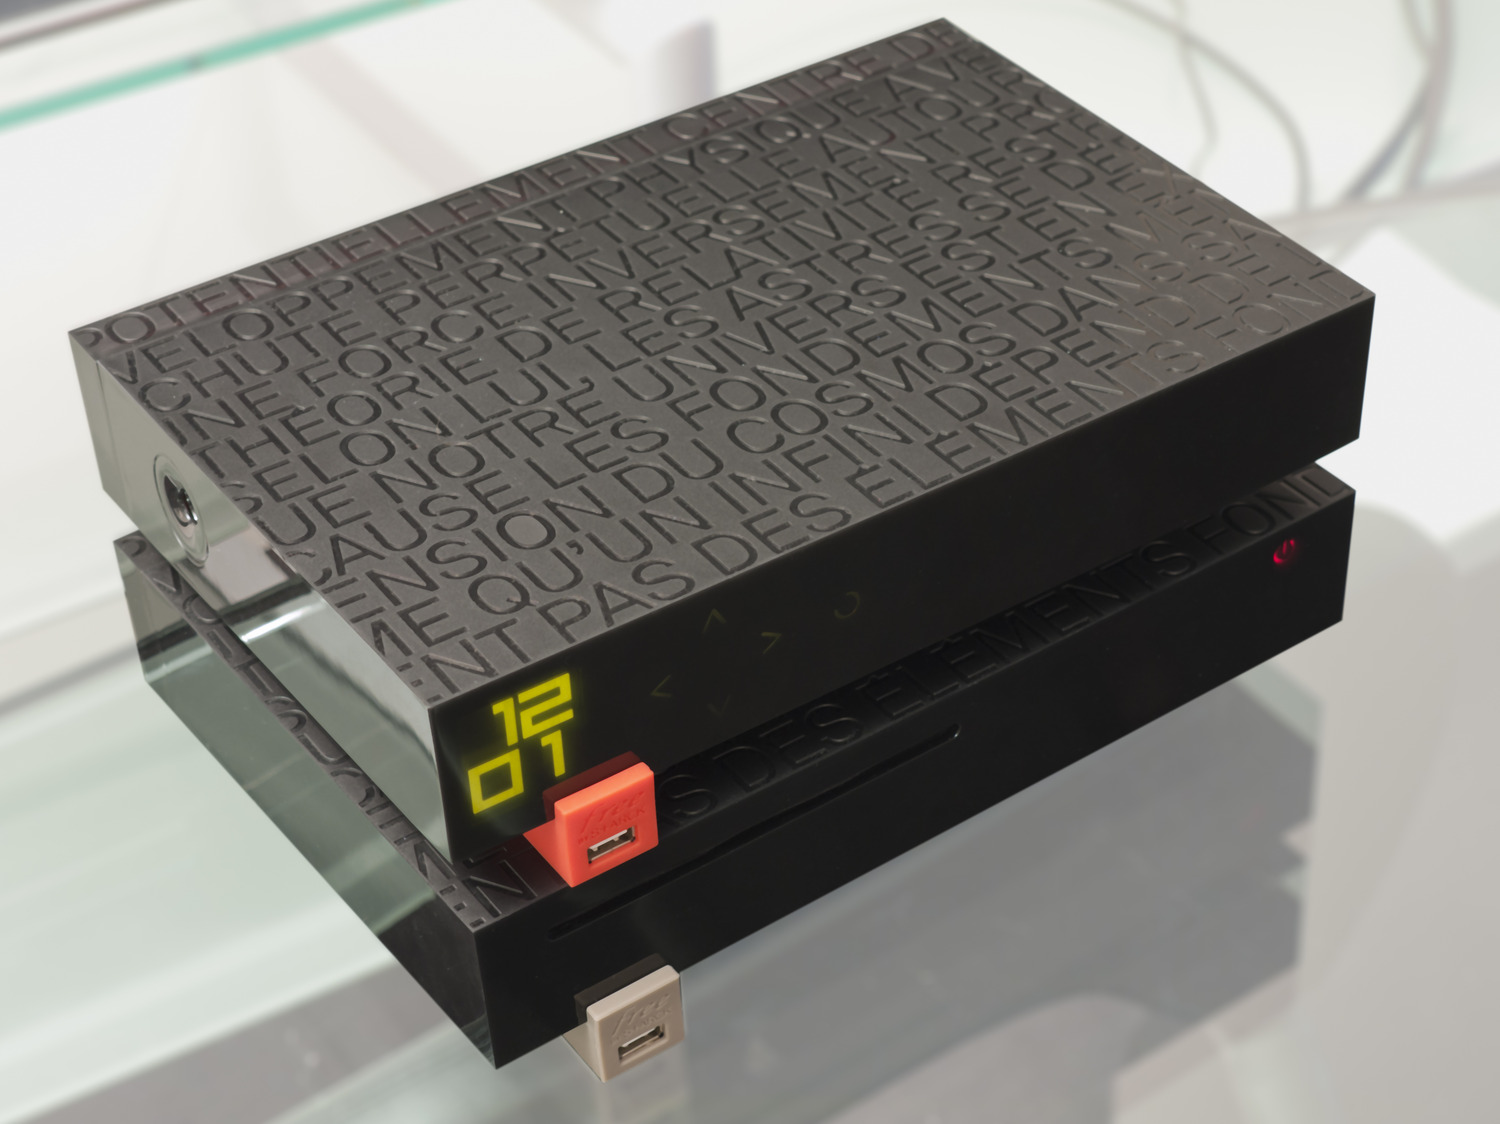
\includegraphics[width=0.7\textwidth]{images/freebox.jpg}
  \end{center}
\end{frame}

\begin{frame}
\frametitle{Televisione}
  \begin{center}
    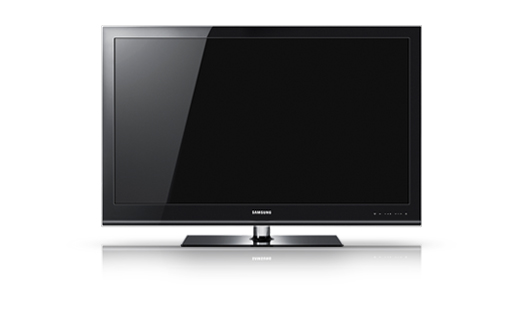
\includegraphics[width=0.7\textwidth]{images/television.jpg}
  \end{center}
\end{frame}

\begin{frame}
\frametitle{Terminale POS}
  \begin{center}
    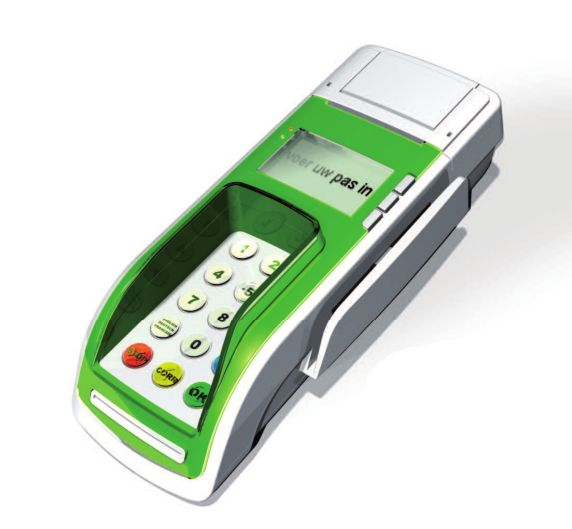
\includegraphics[width=0.7\textwidth]{images/point-of-sale.jpg}
  \end{center}
\end{frame}

\begin{frame}
\frametitle{Tagliatrice laser}
  \begin{center}
    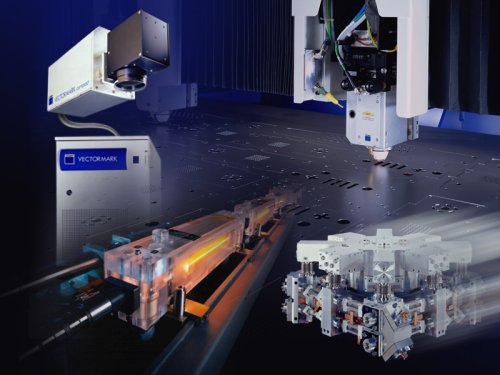
\includegraphics[width=0.7\textwidth]{images/laser-cutting-machine.jpg}
  \end{center}
\end{frame}

\begin{frame}
\frametitle{Stampante 3D}
  \begin{center}
    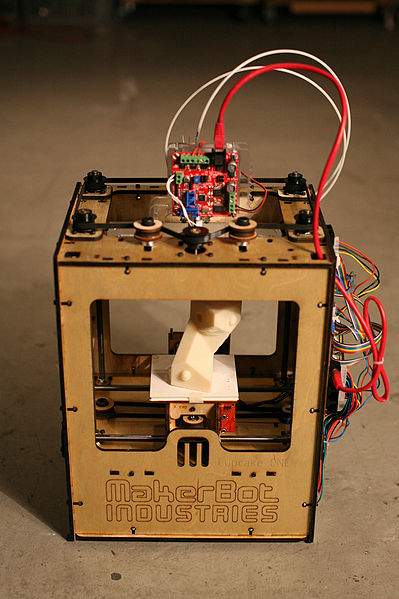
\includegraphics[height=0.8\textheight]{images/3d-printer.jpg}
  \end{center}
\end{frame}

\begin{frame}
  \frametitle{Che cosa è un sistema embedded}
  \begin{itemize}
    \item È un computer
    \item {\color{red} incorporato} in un sistema
    \item programmato per {\color{blue} una specifica applicazione}
    \item con una piattaforma {\color[rgb]{0,0.5,0} hardware ad hoc}
  \end{itemize}
\end{frame}

\begin{frame}
\frametitle{Embedded = piccolo?}
  \begin{center}
    \includegraphics[width=0.9\textwidth]{images/embedded-systems-range.pdf}
  \end{center}
\end{frame}

\begin{frame}
\frametitle{Diffusione di Linux}
  \begin{itemize}
    \item 65\% of smart mobile devices
    \item 95\% of high performance computing market
    \item \textbf{55\% of embedded systems market}
    \item 40\% of enerprise server market
    \item 90\% of world’s stock exchange
  \end{itemize}
  {\tiny Source: Jim Zemlin, State of Linux, LinuxCon 2014,
    \url{https://www.youtube.com/watch?v=YdmT2arOZBw}}
\end{frame}

\begin{frame}
\frametitle{Anatomia di un Sistema Operativo}
  \begin{center}
    \includegraphics[width=0.9\textwidth]{images/system-architecture.pdf}
  \end{center}
\end{frame}

\begin{frame}
\frametitle{Vantaggi di Linux}
  \begin{itemize}
    \item Open Source
    \begin{itemize}
      \item Nessun costo di acquisto (ma vanno rispettate le licenze!)
      \item Esiste una montagna di software pronto da usare
      \item Personalizzabile e adattabile in ogni sua parte
    \end{itemize}
    \item Affidabile
    \item Efficiente
    \item Formato da molti piccoli pezzi
    \begin{itemize}
      \item Quasi nessuno è obbligatorio
      \item Molto sono sostituibili
    \end{itemize}
  \end{itemize}
\end{frame}

\begin{frame}
\frametitle[Demo! Alcuni sistemi Linux embedded in funzione]{Demo}
  \begin{center}
    \LARGE
    Alcuni sistemi embedded Linux in funzione
  \end{center}
\end{frame}

\section{Sfida \#1: Risorse disponibili}

\begin{frame}
\frametitle{Risorse disponibili}
{
  \rowcolors{2}{red!40!blue!40}{red!70!blue!20}
  \begin{tabular}{ |l|c|c|c|  }
    \hline
     & PC & Android & Embedded \\
    \hline
    CPU cores    & 2..8           & 1..4       & 1..8             \\
    CPU clock    & 2..3 GHz       & 1..2 GHz   & 100 MHz .. 3 GHz \\
    RAM          & 4..16 GB       & 1..4 GB    & 8 MB .. 16 GB    \\
    Storage      & 120 GB .. 6 TB & 4..64 GB   & 8 MB .. 1 TB     \\
    Networking   & 1 GB/s, WiFi   & WiFi       & ???              \\
    USB          & 3.0            & 2.0 .. 3.0 & nulla .. 3.0     \\
    \hline
  \end{tabular}
}
\end{frame}

\begin{frame}
\frametitle{Libreria C}
  \begin{columns}
    \column{0.7\textwidth}
    \begin{itemize}
      \item GNU libc: \textasciitilde 2 MB
      \begin{itemize}
        \item La più completa, e conforme agli standard
        \item Usata nelle distribuzioni per PC e server
      \end{itemize}
      \item uClibc-ng: < 1 MB
      \begin{itemize}
        \item Configurabile: si possono disattivare alcuni componenti
          che non servono
      \end{itemize}
      \item musl
      \begin{itemize}
        \item Alternativa recente
        \item Più compatta di uClibc-ng
        \item Configurabile
      \end{itemize}
    \end{itemize}
    \column{0.3\textwidth}
    \includegraphics[width=\textwidth]{images/system-architecture-libc.pdf}
  \end{columns}
\end{frame}

\begin{frame}
\frametitle{Busybox /1}
  \begin{columns}
    \column{0.7\textwidth}
  \begin{spacing}{0}
    \tiny
    \path{[, [[, addgroup, adduser, adjtimex, ar, arp, arping, ash, awk, basename, bbconfig, bbsh, brctl, bunzip2, busybox, bzcat, bzip2, cal, cat, catv, chat, chattr, chcon, chgrp, chmod, chown, chpasswd, chpst, chroot, chrt, chvt, cksum, clear, cmp, comm, cp, cpio, crond, crontab, cryptpw, cttyhack, cut, date, dc, dd, deallocvt, delgroup, deluser, depmod, devfsd, df, dhcprelay, diff, dirname, dmesg, dnsd, dos2unix, dpkg, dpkg_deb, du, dumpkmap, dumpleases, e2fsck, echo, ed, egrep, eject, env, envdir, envuidgid, ether_wake, expand, expr, fakeidentd, false, fbset, fbsplash, fdflush, fdformat, fdisk, fetchmail, fgrep, find, findfs, fold, free, freeramdisk, fsck, fsck_minix, ftpget, ftpput, fuser, getenforce, getopt, getsebool, getty, grep, gunzip, gzip, halt, hd, hdparm, head, hexdump, hostid, hostname, httpd, hush, hwclock, id, ifconfig, ifdown, ifenslave, ifup, inetd, init, inotifyd, insmod, install, ip, ipaddr, ipcalc, ipcrm, ipcs, iplink, iproute, iprule, iptunnel, kbd_mode, kill, killall, killall5, klogd, lash, last, length, less, linux32, linux64, linuxrc, ln, load_policy, loadfont, loadkmap, logger, login, logname, logread, losetup, lpd, lpq, lpr, ls, lsattr, lsmod, lzmacat, makedevs, man, matchpathcon, md5sum, mdev, mesg, microcom, mkdir, mke2fs, mkfifo, mkfs_minix, mknod, mkswap, mktemp, modprobe, more, mount, mountpoint, msh, mt, mv, nameif, nc, netstat, nice, nmeter, nohup, nslookup, od, openvt, parse, passwd, patch, pgrep, pidof, ping, ping6, pipe_progress, pivot_root, pkill, poweroff, printenv, printf, ps, pscan, pwd, raidautorun, rdate, rdev, readahead, readlink, readprofile, realpath, reboot, renice, reset, resize, restorecon, rm, rmdir, rmmod, route, rpm, rpm2cpio, rtcwake, run_parts, runcon, runlevel, runsv, runsvdir, rx, script, sed, selinuxenabled, sendmail, seq, sestatus, setarch, setconsole, setenforce, setfiles, setfont, setkeycodes, setlogcons, setsebool, setsid, setuidgid, sh, sha1sum, showkey, slattach, sleep, softlimit, sort, split, start_stop_daemon, stat, strings, stty, su, sulogin, sum, sv, svlogd, swapoff, swapon, switch_root, sync, sysctl, syslogd, tac, tail, tar, taskset, tcpsvd, tee, telnet, telnetd, test, tftp, tftpd, time, top, touch, tr, traceroute, true, tty, ttysize, tune2fs, udhcpc, udhcpd, udpsvd, umount, uname, uncompress, unexpand, uniq, unix2dos, unlzma, unzip, uptime, usleep, uudecode, uuencode, vconfig, vi, vlock, watch, watchdog, wc, wget, which, who, whoami, xargs, yes, zcat, zcip}
  \end{spacing}
    \column{0.3\textwidth}
    \includegraphics[width=\textwidth]{images/system-architecture-busybox.pdf}
  \end{columns}
\end{frame}

\begin{frame}
\frametitle{Busybox /2}
  \begin{itemize}
    \item Un sistema Linux ha bisogno di molti programmi di base per
      funzionare
      \begin{itemize}
        \item un sistema di init, una shell, un semplice editor di
          testo, programmi per manipolare files, esaminare lo stato
          del sistema, configurare la rete\ldots
      \end{itemize}
    \item In una distribuzione sono tanti eseguibili
      \begin{itemize}
        \item Non pensati per un sistema embedded
        \item Occupano spazio
        \item Diverse fonti, vanno gestiti in modi diversi
      \end{itemize}
    \item Soluzione: Busybox!
      \begin{itemize}
        \item Unico eseguibile, molti programmi
        \item Ottimizzato per un sistema embedded
        \item Molto configurabile
      \end{itemize}
  \end{itemize}
\end{frame}

\begin{frame}
\frametitle{Kernel}
  \begin{columns}
    \column{0.7\textwidth}
    \begin{itemize}
      \item È il nocciolo dell'intero sistema!
      \begin{itemize}
        \item Relativamente piccolo ma estremamente importante
        \item Grande potere (e grande responsabilità!)
      \end{itemize}
      \item {\bf Gestisce tutte le risorse hardware}: CPU, memoria, I/O\ldots
      \item Fornisce un'interfaccia {\bf portabile} all'hardware per le
        librerie ed applicazioni
      \item È mostruosamente configurabile
    \end{itemize}
    \column{0.3\textwidth}
    \includegraphics[width=\textwidth]{images/system-architecture-kernel.pdf}
  \end{columns}
\end{frame}

\begin{frame}
\frametitle[Demo! Configurazione del kernel]{Demo}
  \begin{center}
    \LARGE
    Configurazione del kernel
  \end{center}
\end{frame}

\section{Sfida \#2: Cross-compilazione}

\begin{frame}
\frametitle{Architettura delle CPU}
  \begin{center}
    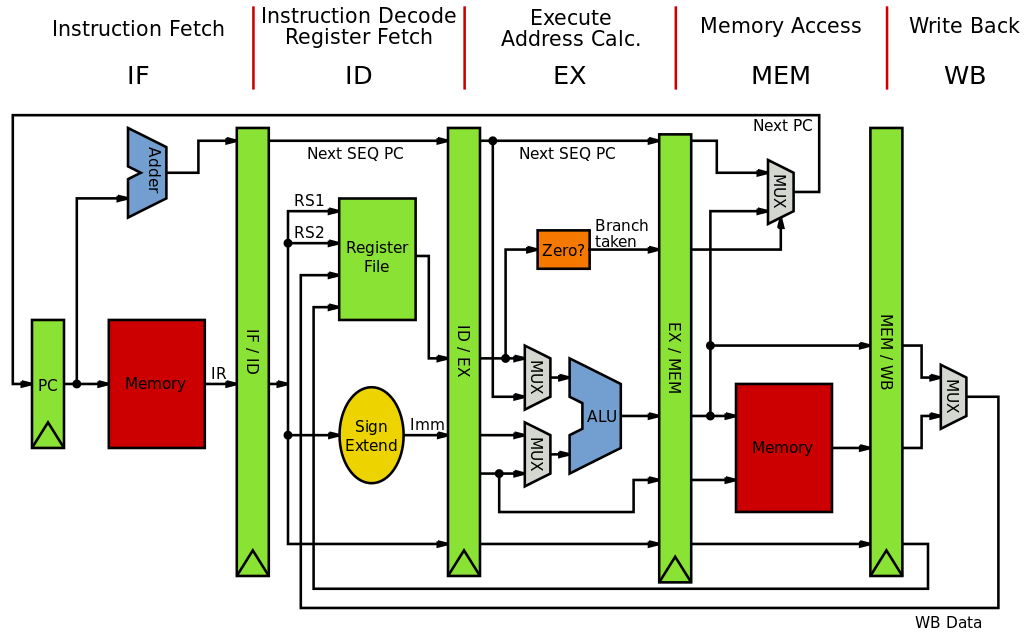
\includegraphics[height=0.6\textheight]{images/mips-architecture.png}\\
    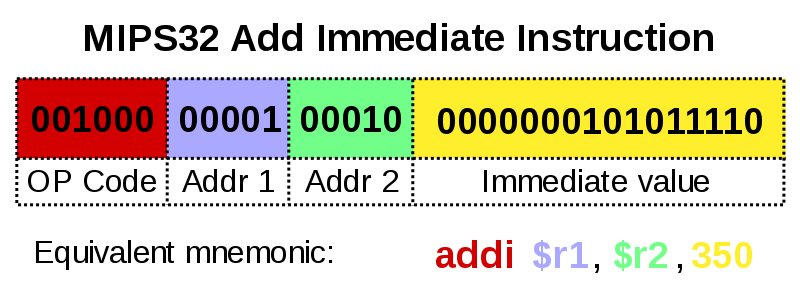
\includegraphics[height=0.2\textheight]{images/mips32-instruction.png}
  \end{center}
\end{frame}

\begin{frame}
\frametitle{Host VS Target}
  \begin{center}
    \includegraphics[height=0.6\textheight]{images/global-architecture.pdf}
  \end{center}
\end{frame}

\begin{frame}
\frametitle{Toolchain}
  \begin{itemize}
  \item Toolchain = strumenti per tradurre i sorgenti in eseguibili e
    librerie = compilatore + linker + altri strumenti
  \item Il compilatore standard del PC è una {\bf toolchain nativa}
    \begin{itemize}
    \item è un programma x86 che gira sul PC
    \item produce un programma x86 che gira sul PC
    \end{itemize}
  \item Per un sistema embedded (non x86) serve una {\bf cross
    toolchain}
    \begin{itemize}
    \item è un programma x86 che gira sul PC (``host'')
    \item produce un programma ARM, MIPS... che gira sul sistema
      embedded (``target'')
    \end{itemize}
  \end{itemize}
\end{frame}

\begin{frame}
\frametitle{Come mi procuro una cross-toolchain?}
  \begin{itemize}
  \item Fai da te (e buona fortuna!)
  \item crosstool-NG
  \item Openembedded
  \item Buildroot
  \item Toolchain già pronta
  \end{itemize}
\end{frame}

\begin{frame}
\frametitle[Demo! Cross-compilazione]{Demo}
  \begin{center}
    \LARGE
    Cross-compilazione
  \end{center}
\end{frame}

\section{Sfida \#3: Comporre un puzzle}

\begin{frame}
\frametitle{Sistemi operativi standardizzati}
  \begin{itemize}
  \item Distribuzioni Linux, Windows, Android...
  \item Molte librerie e servizi di base sempre presenti
  \item Le applicazioni possono contare su un ambiente sempre uguale
  \end{itemize}
\end{frame}

\begin{frame}
\frametitle{Sistemi embedded Linux}
  \begin{itemize}
  \item Probabilmente c'è dell'hardware in meno
    \begin{itemize}
    \item Non è detto che ci siano schermo, tastiera, mouse,
      touchscreen
    \end{itemize}
  \item Probabilmente c'è dell'hardware in più
    \begin{itemize}
    \item Controllo motori, lettore di carte magnetiche,
      telecomando, pannelli LED a scritta variabile\ldots
    \end{itemize}
  \item Non si può dar per scontato di avere librerie e servizi di
    base come su PC
  \item Spesso vanno realizzati in modo sartoriale
  \item Bisogna trovare i pezzi, sceglierli, assemblarli\ldots
    \begin{itemize}
    \item Possono essere molti
    \item Può essere difficile farli cooperare correttamente
    \end{itemize}
  \end{itemize}
\end{frame}

\begin{frame}
\frametitle{Come assemblare i pezzi}
  \begin{itemize}
  \item Fai da te (e buona fortuna!)
  \item Build system
    \begin{itemize}
    \item Buildroot
    \item Openembedded
    \item OpenWRT
    \item \ldots
    \end{itemize}
  \item Distribuzioni embedded pronte
    \begin{itemize}
    \item Utilizzabile solo con hardware relativamente potente
    \end{itemize}
  \end{itemize}
\end{frame}

\begin{frame}
\frametitle{Buildroot}
  \begin{itemize}
  \item Buildroot --- Making Embedded Linux Easy
  \item Strumento per generare tutti i componenti
    \begin{itemize}
    \item Cross-toolchain
    \item Bootloader
    \item Kernel
    \item Root filesystem: librerie, applicativi\ldots
      \begin{itemize}
      \item Contiene le ``ricette'' per compilare oltre 1700 pacchetti
      \end{itemize}
    \item File ``immagine'' scrivere in flash, SD\ldots
    \end{itemize}
  \item \url{http://buildroot.net/}
  \end{itemize}
\end{frame}

\begin{frame}
  \frametitle{Buildroot: configurazione}
  \begin{columns}
    \column{0.6\textwidth}
    \begin{itemize}
    \item Si configura con \path{kconfig} come il kernel:\\
      \texttt{make menuconfig}
    \item Permette di definire
      \begin{itemize}
      \item L'architettura della CPU
      \item Le caratteristiche della toolchain
      \item Le applicazioni e librerie includere
      \item I tipi di file immagine da generare
      \item La configurazione del kernel
      \item La configurazione del bootloader
      \end{itemize}
    \end{itemize}
    \column{0.4\textwidth}
    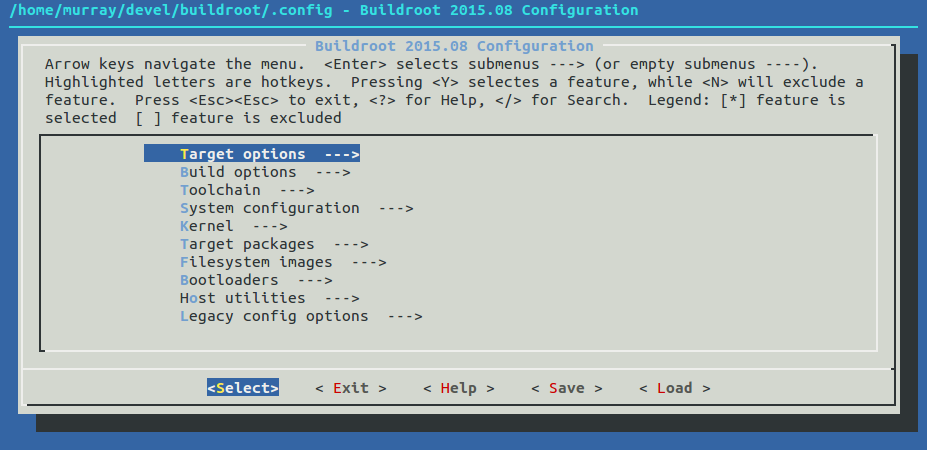
\includegraphics[width=\textwidth]{images/buildroot.png}
  \end{columns}
\end{frame}

\begin{frame}
  \frametitle{Buildroot: esecuzione}
  \begin{columns}
    \column{0.5\textwidth}
    \begin{itemize}
    \item Per compilare il tutto:\\
      \texttt{make}
    \item Per ciascun pacchetto esegue diversi passi:
      \begin{itemize}
      \item Download dei sorgenti
      \item Extract
      \item Patch
      \item Configure
      \item Build
      \item Install
      \end{itemize}
    \item Alle fine genera l'immagine di root filesystem, kernel e
      quant'altro necessario
    \end{itemize}
    \column{0.5\textwidth}
    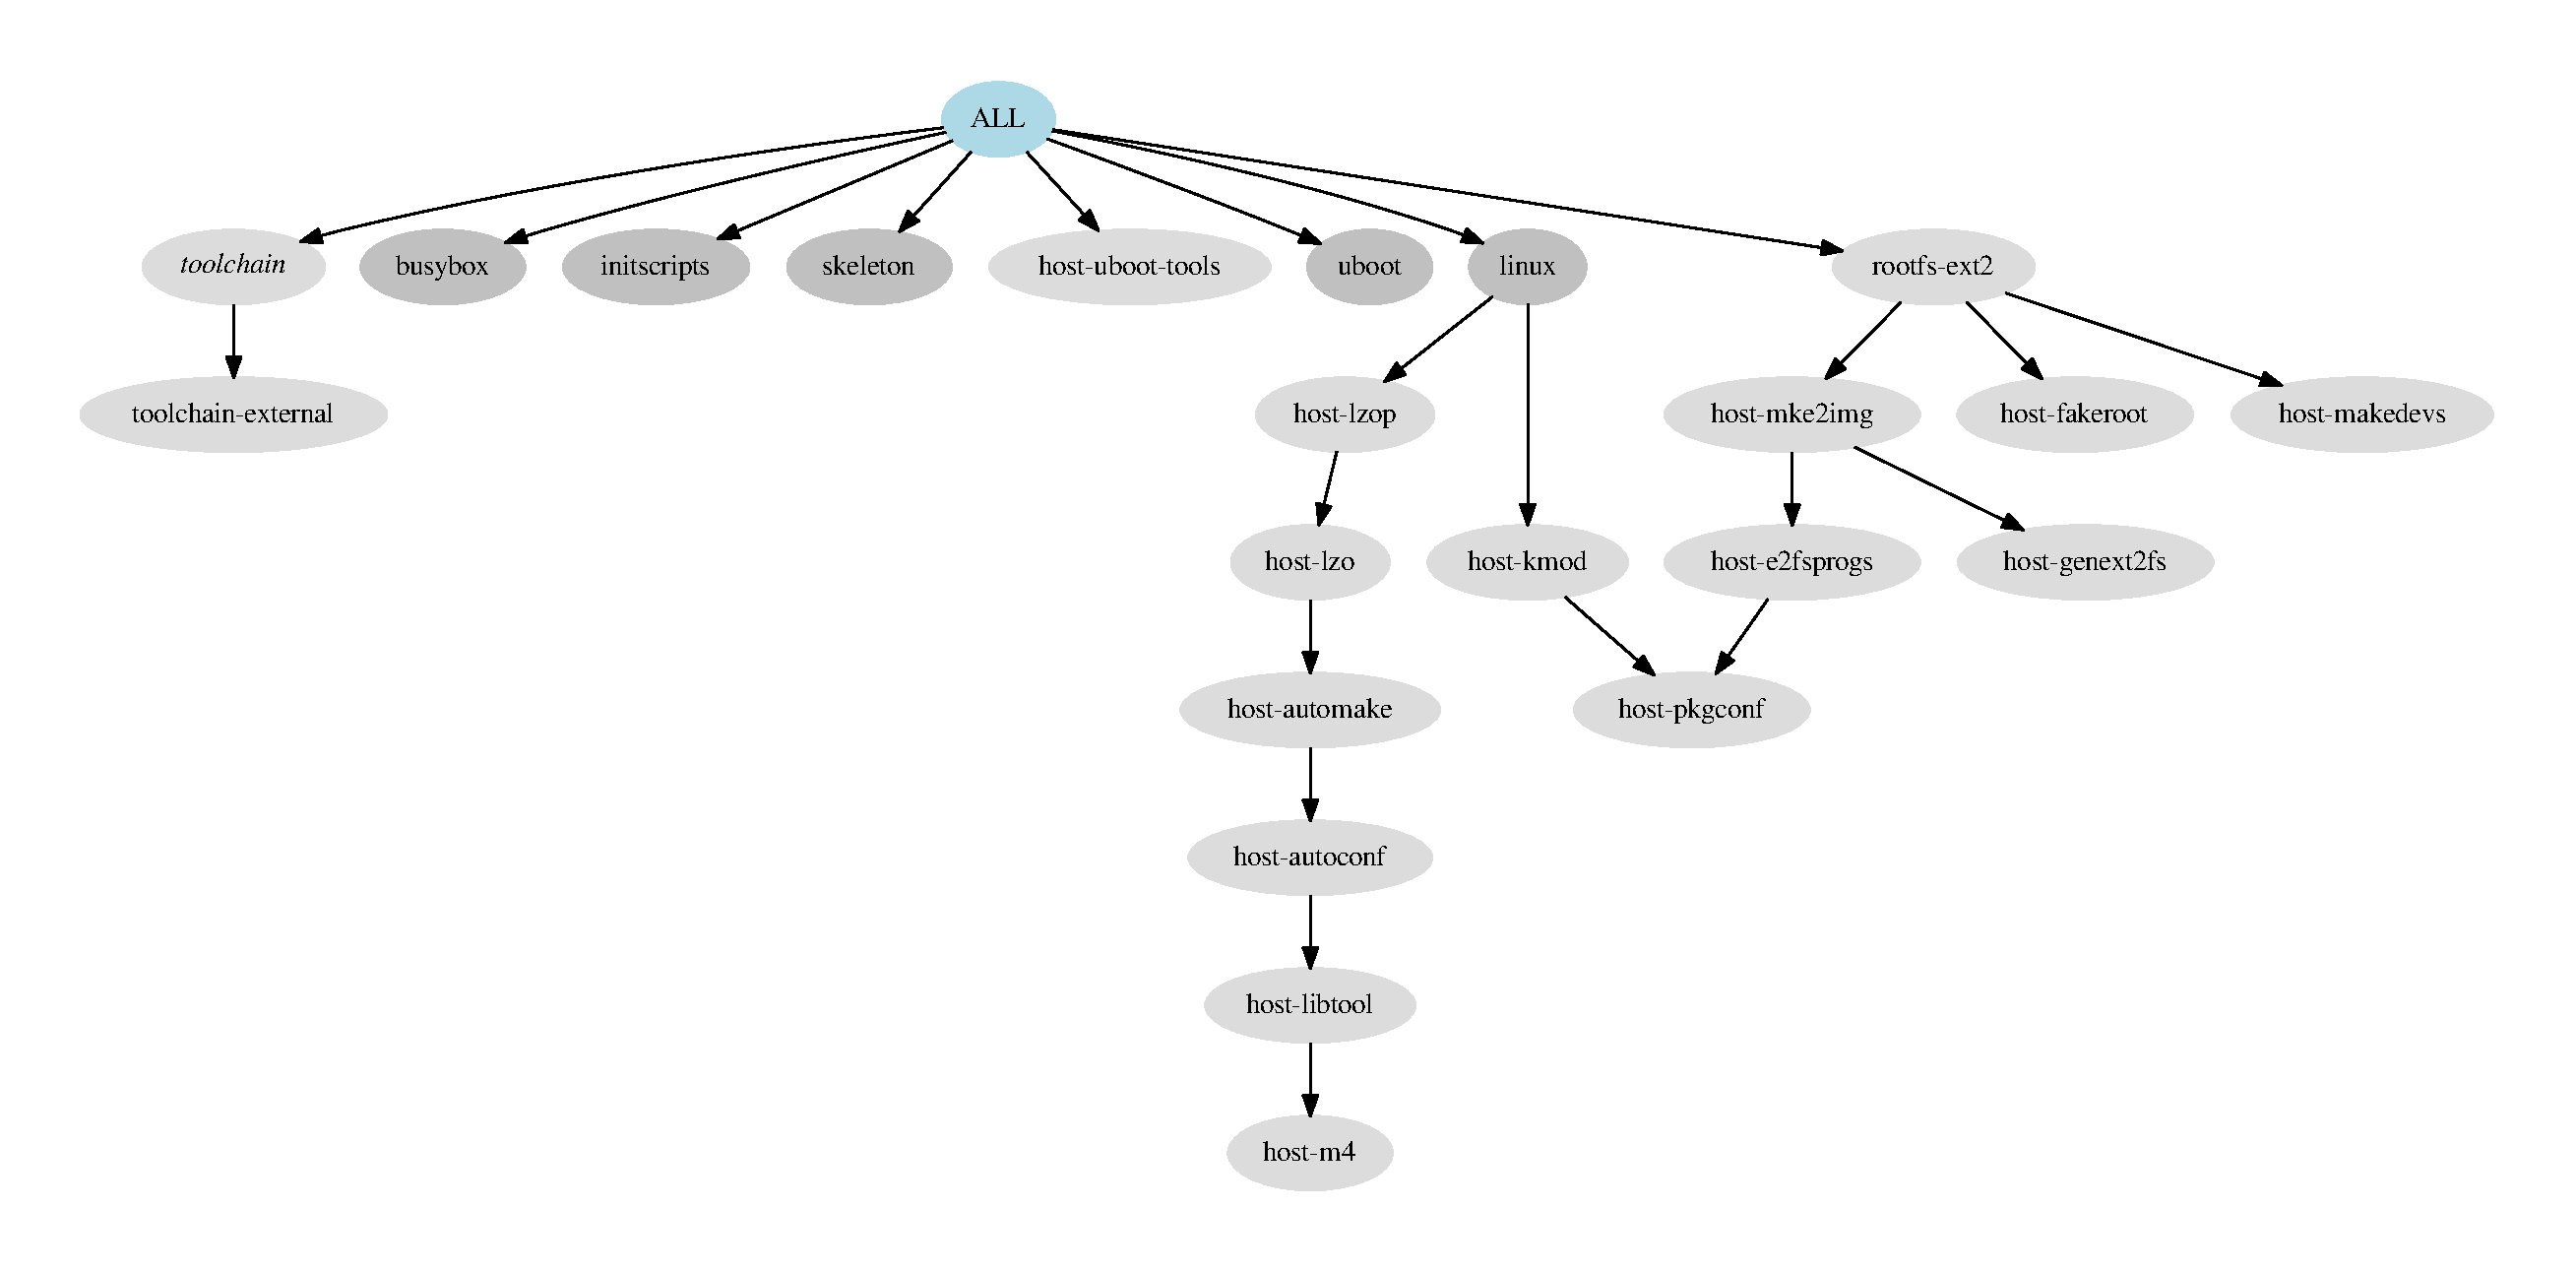
\includegraphics[width=\textwidth]{images/graph-depends.pdf}
  \end{columns}
\end{frame}

\begin{frame}
\frametitle[Demo! Da zero a login con Buildroot]{Demo}
  \begin{center}
    \LARGE
    Da zero a login con Buildroot
  \end{center}
\end{frame}

\begin{frame}
\frametitle{Fine}

  \begin{center}
    {\Huge Domande?}

    \vspace{0.1\textheight}

    © Copyright 2015, Luca Ceresoli\\
    \href{mailto:luca@lucaceresoli.net}{luca@lucaceresoli.net}\\
    \url{http://www.lucaceresoli.net}

  \vspace{0.05\textheight}

   \tiny
   Materiale rlasciato sotto
   licenza Creative Commons Attribution - Share Alike 3.0 \\
   \url{https://creativecommons.org/licenses/by-sa/3.0/legalcode} \\
  \end{center}

  \vspace{0.05\textheight}

  Materiale da:

  \vspace{0.01\textheight}
  \begin{tiny}
    {
      \setlength{\parskip}{0cm plus0mm minus3mm}
      \fontsize{4}{0}
      \url{http://free-electrons.com/doc/training/embedded-linux/}\\
      \url{https://en.wikipedia.org/wiki/File:Mips32_addi.svg}\\
      \url{https://en.wikipedia.org/wiki/File:MIPS_Architecture_(Pipelined).svg}\\
      \url{https://commons.wikimedia.org/wiki/File:NN-K125MBGPG_Grill-Mikrowelle_silber_Panasonic.png}\\
      \url{https://commons.wikimedia.org/wiki/File:Bancomat_ATM_italy.jpg}\\
      \url{https://commons.wikimedia.org/wiki/File:MakerBot_ThingOMatic_Bre_Pettis.jpg}\\
    }
  \end{tiny}
\end{frame}

\end{document}
